\documentclass{article}
\usepackage{graphicx}
\usepackage{amsmath,amsthm,amssymb}
\usepackage[font=small,labelfont=bf]{caption}
\usepackage{tikz}
\usetikzlibrary{calc, angles, quotes, shapes.geometric, decorations.pathreplacing}
\usepackage{tkz-euclide}
\usepackage[inline]{asymptote}
\usepackage{float}
\usepackage[margin=1in]{geometry}
\usepackage{gensymb}
\usepackage[normalem]{ulem}
\usepackage{hyperref}
\hypersetup{
    colorlinks=true,
    linkcolor=blue,
    filecolor=magenta,      
    urlcolor=cyan,
    pdftitle={Overleaf Example},
    pdfpagemode=FullScreen,
    }
\usepackage{fancyhdr}
\pagestyle{fancy}
\fancyhead[R]{Enoch Yu}
\pagenumbering{gobble}
\usepackage{enumitem}
\newtheorem{theorem}{Theorem}[section]
\newtheorem{lemma}[theorem]{Lemma}
\newtheorem*{lemma*}{Lemma}
\newtheorem{sublemma}{Lemma}[section]
\newtheorem{proposition}{Proposition}
\newtheorem{corollary}{Corollary}[theorem]
\newtheorem{example}{Example}[section]
\newtheorem*{example*}{Example}
\newenvironment{solution}{\begin{trivlist}\item[]{\bf Solution}}{\qed \end{trivlist}}
\newcommand{\verteq}{\rotatebox{90}{$\;\;=\;\;$}}
\newcommand*\circled[1]{\tikz[baseline=(char.base)]{
            \node[shape=circle,draw,inner sep=1pt] (char) {#1};}}
\newcommand{\triangled}[1]{\tikz[baseline=(char.base)]{
            \node[shape=regular polygon, regular polygon sides=3, draw, inner sep=0.2pt] (char) {#1};}}

\title{Problem Set 21}
\author{Enoch Yu}
\date{June 2025}

\begin{document}

\section*{Problem}
If $S = \frac{1}{\frac{1}{1980} + \frac{1}{1981} + \dots + \frac{1}{1997}}$, what is the integer part of $S$?
\begin{solution}
\\\\
\textbf{Key Word} Properties of Fraction
\\\\
First and foremost, when the range of the denominator could be found, the range of $S$ would also be obtained. Let $S' = \frac{1}{1980} + \frac{1}{1981} + \dots + \frac{1}{1997}$
\begin{align*}
    \frac{1}{1980} + \dots + \frac{1}{1980} >\ &S' > \frac{1}{1997} + \dots + \frac{1}{1997} \\
    \frac{18}{1980} >\ &S' > \frac{18}{1997} \\
    \frac{1}{\frac{18}{1980}} <\ &S < \frac{1}{\frac{18}{1997}} \\
    \frac{1980}{18} <\ &S < \frac{1997}{18} \\
    110 <\ &S < 110.9444
\end{align*}
Therefore, the integer part of $S$ is $\boxed{110}$.
\end{solution}

\newpage
\section*{2021 Fall AMC 12A Problem 21}
Let $ABCD$ be an isosceles trapezoid with $\overline{BC} \parallel \overline{AD}$ and $AB=CD$. Points $X$ and $Y$ lie on diagonal $\overline{AC}$ with $X$ between $A$ and $Y$, as shown in the figure. Suppose $\angle AXD = \angle BYC = 90^\circ$, $AX = 3$, $XY = 1$, and $YC = 2$. What is the area of $ABCD$?

\begin{center}
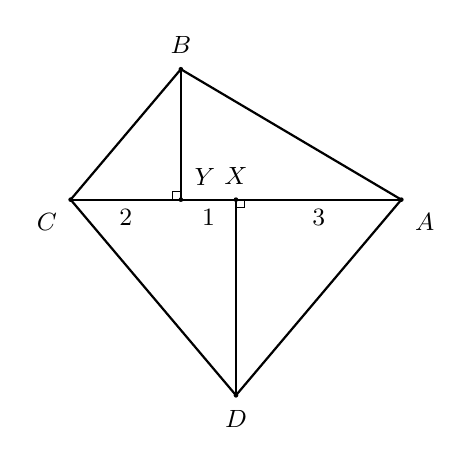
\begin{tikzpicture}[scale=0.7, every node/.style={font=\small}]
    \coordinate (C) at (0,0);
    \coordinate (Y) at (2,0);
    \coordinate (X) at (3,0);
    \coordinate (A) at (6,0);
    \coordinate (B) at (2,{sqrt(5.6)});
    \coordinate (D) at (3,{-sqrt(12.6)});

    \draw[thick] (A) -- (B) -- (C) -- (D) -- cycle;
    \draw[thick] (A) -- (C);
    \draw[thick] (B) -- (Y);
    \draw[thick] (D) -- (X);

    \foreach \pt in {A,B,C,D,X,Y}
        \fill[black] (\pt) circle (1.2pt);

    \node[below left=2pt] at (C) {$C$};
    \node[below right=2pt] at (A) {$A$};
    \node[above=2pt] at (B) {$B$};
    \node[below=2pt] at (D) {$D$};
    \node[above=2pt] at (X) {$X$};
    \node[above right=2pt] at (Y) {$Y$};

    \node[below] at ($(C)!0.5!(Y)$) {$2$};
    \node[below] at ($(Y)!0.5!(X)$) {$1$};
    \node[below] at ($(X)!0.5!(A)$) {$3$};

    \tkzMarkRightAngle[size=.15](C,Y,B);
    \tkzMarkRightAngle[size=.15](D,X,A);
\end{tikzpicture}
\end{center}
$\textbf{(A)}\: 15\qquad\textbf{(B)} \: 5\sqrt{11}\qquad\textbf{(C)} \: 3\sqrt{35}\qquad\textbf{(D)} \: 18\qquad\textbf{(E)} \: 7\sqrt{7}$

\begin{solution}
\\\\
\textbf{Key Word} Pythagorean Theorem
\\\\
First, different ratios and relationships could be found through the diagram.
\begin{center}
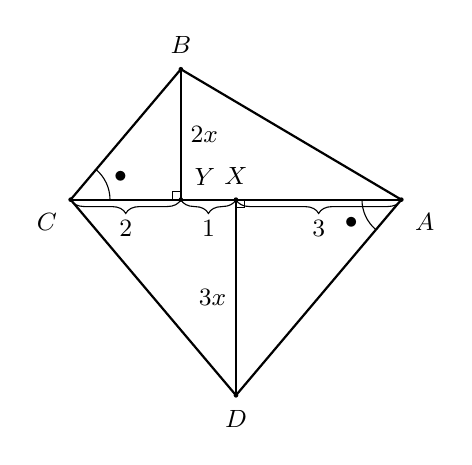
\begin{tikzpicture}[scale=0.7, every node/.style={font=\small}]
    \coordinate (C) at (0,0);
    \coordinate (Y) at (2,0);
    \coordinate (X) at (3,0);
    \coordinate (A) at (6,0);
    \coordinate (B) at (2,{sqrt(5.6)});
    \coordinate (D) at (3,{-sqrt(12.6)});

    \draw[thick] (A) -- (B) -- (C) -- (D) -- cycle;
    \draw[thick] (A) -- (C);
    \draw[thick] (B) -- (Y);
    \draw[thick] (D) -- (X);

    \foreach \pt in {A,B,C,D,X,Y}
        \fill[black] (\pt) circle (1.2pt);

    \node[below left=2pt] at (C) {$C$};
    \node[below right=2pt] at (A) {$A$};
    \node[above=2pt] at (B) {$B$};
    \node[below=2pt] at (D) {$D$};
    \node[above=2pt] at (X) {$X$};
    \node[above right=2pt] at (Y) {$Y$};

    \draw[decorate,decoration={brace,mirror,amplitude=5pt},yshift=-2pt]
        (C) -- (Y) node[midway,below=4pt] {\small 2};
    \draw[decorate,decoration={brace,mirror,amplitude=5pt},yshift=-2pt]
        (Y) -- (X) node[midway,below=4pt] {\small 1};
    \draw[decorate,decoration={brace,mirror,amplitude=5pt},yshift=-2pt]
        (X) -- (A) node[midway,below=4pt] {\small 3};

    \tkzMarkRightAngle[size=.15](C,Y,B);
    \tkzMarkRightAngle[size=.15](D,X,A);

    \draw pic["$\bullet$", draw=black, angle radius=0.5cm, angle eccentricity=1.4] {angle=Y--C--B};
    \draw pic["$\bullet$", draw=black, angle radius=0.5cm, angle eccentricity=1.4] {angle=X--A--D};

    \node[right] at ($(B)!0.5!(Y)$) {$2x$};
    \node[left] at ($(D)!0.5!(X)$) {$3x$};
\end{tikzpicture}
\end{center}
Using the Pythagorean Theorem, the following equations are true.
\begin{align*}
    (2x)^2 + 4^2 &= 3^2 + (3x)^2 \\
    4x^2 + 16 &= 9 + 9x^2 \\
    5x^2 &= 7 \\
    x^2 &= \frac{7}{5}
    \\\\
    \frac{1}{2} \cdot 6 \cdot 5x
    &= 15 \cdot \sqrt{\frac{7}{5}} \\
    &= \boxed{\textbf{(C)} \: 3\sqrt{35}}
\end{align*}
\end{solution}

\newpage
\section*{2021 Fall AMC 12A Problem 23}
A quadratic polynomial with real coefficients and leading coefficient $1$ is called $\emph{disrespectful}$ if the equation $p(p(x))=0$ is satisfied by exactly three real numbers. Among all the disrespectful quadratic polynomials, there is a unique such polynomial $\tilde{p}(x)$ for which the sum of the roots is maximized. What is $\tilde{p}(1)$?
\\\\
$\textbf{(A) } \frac{5}{16} \qquad\textbf{(B) } \frac{1}{2} \qquad\textbf{(C) } \frac{5}{8} \qquad\textbf{(D) } 1 \qquad\textbf{(E) } \frac{9}{8}$

\begin{solution}
\\\\
\textbf{Key Word} Graphing Quadratic Functions
\\\\
Because $p(x)$ is a quadratic equation with a leading coefficient of 1, let $p(x) = x^2 + ax + b$. Moreover, let $r_1, r_2, r_3$ be the roots of the equation $p(p(x)) = 0$.
\begin{align*}
    p(r_1) &= a \\
    p(r_2) &= b \\
    p(r_3) &= c
    \\\\
    p(a) = p(b) &= p(c) = 0 \\
    p(x) &= (x - \alpha)(x - \beta)
\end{align*}
The following cases are the possible graphs for $p(x)$.
\begin{center}
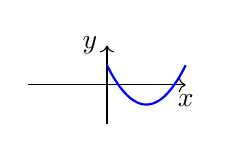
\begin{tikzpicture}[scale=0.5]
  \draw[->] (-2,0) -- (2,0) node[below] {$x$};
  \draw[->] (0,-1) -- (0,1) node[left] {$y$};
  
  \draw[domain=0:2, smooth, variable=\x, blue, thick] 
    plot ({\x}, {\x*\x - 2*\x + 0.5});
\end{tikzpicture}
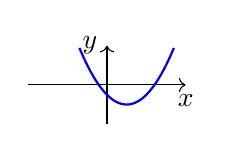
\begin{tikzpicture}[scale=0.5]
  \draw[->] (-2,0) -- (2,0) node[below] {$x$};
  \draw[->] (0,-1) -- (0,1) node[left] {$y$};
  
  \draw[domain=-0.7:1.7, smooth, variable=\x, blue, thick] 
    plot ({\x}, {\x*\x - \x - 0.25});
\end{tikzpicture}
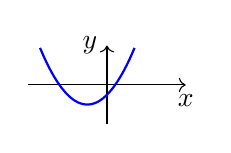
\begin{tikzpicture}[scale=0.5]
  \draw[->] (-2,0) -- (2,0) node[below] {$x$};
  \draw[->] (0,-1) -- (0,1) node[left] {$y$};
  
  \draw[domain=-1.7:0.7, smooth, variable=\x, blue, thick] 
    plot ({\x}, {\x*\x + \x - 0.25});
\end{tikzpicture}
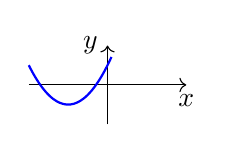
\begin{tikzpicture}[scale=0.5]
  \draw[->] (-2,0) -- (2,0) node[below] {$x$};
  \draw[->] (0,-1) -- (0,1) node[left] {$y$};
  
  \draw[domain=-2:0.1, smooth, variable=\x, blue, thick] 
    plot ({\x}, {\x*\x + 2*\x + 0.5});
\end{tikzpicture}
\end{center}
The second graph is the case that could provide the maximum sum of the roots.
\begin{align*}
    \therefore \left( x - \frac{\alpha + \beta}{2} \right)^2 + \alpha &= (x - \alpha)(x - \beta) \\
    x^2 - (\alpha + \beta)x + \frac{(\alpha + \beta)^2}{4} + \alpha &= x^2 - (\alpha + \beta)x + \alpha\beta \\
    \frac{(\alpha + \beta)^2}{4} + \alpha &= \alpha\beta \\
    (\alpha + \beta)^2 &= 4\alpha\beta - 4\alpha = 4\alpha(\beta - 1)
    \\\\
    \sqrt{\alpha(\beta - 1)} &\le \frac{\alpha + (\beta - 1)}{2} \\
    &leads\ to \\
    \alpha &= \beta - 1.
    \\\\
    (\alpha + \beta)^2 &= 4\alpha^2 \\
    \alpha = \beta\ &or\ 3\alpha + \beta = 0
    \\\\
    \therefore \alpha = -\frac{1}{4}&, \beta = \frac{3}{4}
    \\\\
    p(1) = (1 - \alpha)(1 - \beta) &= \frac{5}{4} \cdot \frac{1}{4} = \boxed{\textbf{(A) } \frac{5}{16}}
\end{align*}
\end{solution}
Uploaded a \href{https://artofproblemsolving.com/wiki/index.php/2021_Fall_AMC_12A_Problems/Problem_23#Solution_11_.28AM-GM_Inequality.29}{new solution} in AOPS!! \\
\includegraphics[scale=0.6]{Screenshot 2025-06-18 at 5.27.30 PM.png}

\end{document}
